
%\documentclass[a4paper]{jsbook}
%\usepackage{mcmd_jp}
%\begin{document}

\section{mcal 項目間演算\label{sect:mcal}}
\index{mcal@mcal}

\verb|c=|パラメータで指定した計算式で計算をおこない、\verb|a=|パラメータで指定した項目名に出力する。
\verb|mcal|が出力する項目は、プログラムの単純化のため、例外なく1つに限定している。
計算式の詳細は後述の「式の構成要素」を参照のこと。

\subsection*{書式}
\verb|mcal a= c=|
\hyperref[sect:option_i]{[i=]}
\hyperref[sect:option_o]{[o=]}
\hyperref[sect:option_assert_diffSize]{[-assert\_diffSize]}
\hyperref[sect:option_assert_nullout]{[-assert\_nullout]}
\hyperref[sect:option_nfn]{[-nfn]} 
\hyperref[sect:option_nfno]{[-nfno]}  
\hyperref[sect:option_x]{[-x]}
\hyperref[sect:option_option_tmppath]{[tmpPath=]}
\hyperref[sect:option_precision]{[precision=]}
\verb|[-params]|
\verb|[--help]|
\verb|[--helpl]|
\verb|[--version]|\\

\subsection*{パラメータ}
\begin{table}[hb]
%\begin{center}
{\small
\begin{tabular}{ll}
\verb|i=|    & 入力ファイル名を指定する。\\
\verb|o=|    & 出力ファイル名を指定する。\\
\verb|a=|    & 新たに計算結果の出力として追加される項目の名前を指定する。\\
\verb|c=|    & 用意された関数を組み合わせて計算する式を指定する。\\
\end{tabular} 
}
\end{table} 

\subsection*{利用例}
以下に\verb|mcal|を使った簡単な例を示す。
個々の関数や演算子についての詳細は、それぞれ個別に解説を用意しているので、そちらを参照されたい。

\begin{Verbatim}[baselinestretch=0.7,frame=single,fontsize=\small]
# 入力ファイル(dat1.csv)
顧客,数量,単価
A,3,10
B,1,15
C,2,20

$ mcal c='${数量}*${単価}' a=金額 i=dat1.csv
顧客,数量,単価,金額
A,3,10,30
B,1,15,15
C,2,20,40

$ mcal c='${数量}*${単価}<=30' a=金額30以下 i=dat1.csv
顧客,数量,単価,金額30以下
A,3,10,1
B,1,15,1
C,2,20,0

$ mcal c='if(top(),${単価},#{}+${単価})' a=単価累計 i=dat1.csv
顧客,数量,単価,単価累計
A,3,10,10
B,1,15,25
C,2,20,45
\end{Verbatim}


%\subsection*{データ形式}
%mcalは用意された関数を組合せて柔軟な計算を行うことができるコマンドである。\\
%その際、入出力のデータの型には注意する必要がある。\\
%例えば2008年8月15日を"20080815"と表している日付データに対して、
%17日を加えると結果は"20080901"となるが、数値として17を加えると結果は"20080832"となるからである。\\
%mcalには、数値、文字、日付("20080815"など)、時刻("20080815235959"など)、
%論理("真"あるいは"偽")の5つの型がある。\\

\subsection*{シェルでの利用時の注意事項}
UNIX系のOSでbashなどのシェルを利用する場合、演算子などの記号はシェルにとっても特殊な意味を持つことが多い。
例えば\verb|$|記号に続く単語列はシェル変数を意味する。
一方でmcmdでは項目値を参照するために\verb|$|を使っている。
そこでシェルにそれらの記号を解釈させないために、以下のようにシングルクオーツで囲む必要がある。

\verb|$ mcal c='${date}-10'|

\subsection*{エラーメッセージ}

\verb|#ERROR# unknown function or operator|

このエラーメッセージが出るということは、関数もしくは演算子の指定に誤りがある。
例えば、以下のような文字列の結合関数catについてのエラーメッセージについて考える。

\begin{Verbatim}[baselinestretch=0.7,frame=single,fontsize=\small]
 $ mcal c='cat("-",1,2)'
 ERROR : unknown function or operator: cat_SNN(cat_SN) (kgcal)
\end{Verbatim}

「cat\_SNN」のアンダーバーの前のcatは関数名を示し、その後のSNNは引数の型を示している。
Sは文字列型、Nは数字型、Dは日付型、Tは時刻型、Bは真偽型である。
3つの引数を指定しているので3文字(SNN)となっている。
すなわち、このエラーメッセージは「引数としてSNNをとるcatという名前の関数」
は登録されていないということを意味する。
以下のように2,3番目の引数を文字列型にすればよい。
\begin{Verbatim}[baselinestretch=0.7,frame=single,fontsize=\small]
 $ mcal c='cat("-","1","2")'
\end{Verbatim}

ここで、エラーメッセージの括弧の中は2文字(SN)となっているが、それは2番目以降のパラメータが可変個指定可能であるため、
それらの代表として1つだけ表記しているためである。

%\begin{Verbatim}[baselinestretch=0.7,frame=single,fontsize=\small]
%$ mcal c='cat(${商品ID},${単価},"-")' a=商品ID-単価 i=dat1.csv o=rsl1.csv
%\end{Verbatim}

\subsection*{関連コマンド}
\hyperref[sect:msel]{msel} : 演算の結果を用いて行選択するのであればこのコマンドを使う。



\section{式の構成要素\label{sec:elem}}
\verb|mcal|で記述する式を構成する要素は、定数、項目値、演算子、関数の4つに大きく分類できる。
そして、それぞれの要素において、ユーザはデータ型を意識して利用する必要がある。
mcalが扱うデータはCSVテキストなので、値は全て文字列として与えらており、
それら文字列を\verb|mcal|でどのようなデータ型として扱うかはユーザに委ねられているからである。
mcalが規定するデータ型は文字列型($str$),数値型($num$)、日付型($date$)、時刻型($time$)、論理型($bool$)の5つである。
以下では、式を構成するそれぞれの要素で、5つのデータ型をどのように扱うかを示す。

\section{定数}
\begin{table}[!hb]
\begin{center}
\caption{定数の書式一覧}
{\small
  \begin{tabular}{l|l|l|l} \hline
データ型&書式&内容&例\\ \hline
数値($num$)   & 整数、実数の文字列表記& 内部的には全て倍精度実数を利用           & \verb|20, 0.55, 1.5*e10|\\
文字列($str$) & "文字列"         & ダブルクオーテーションで括った文字列          & \verb|"abc" "日本語"|\\
日付($date$)  & 0dyyyymmdd       & 先頭に"0d"を付けた年月日固定長                & \verb|0d20080923| \\
時刻($time$)  & 0tyyyymmddHHMMSS & 先頭に"0t"を付けた年月日時分秒固定長          & \verb|0t20080923121115|\\
              & 0tHHMMSS         & 先頭に"0t"を付けた時分秒固定長                & \verb|0t121115|\\
              &                  & (内部的に本日の日付が補完される)              & \\
論理($bool$)  & 0b1, 0b0         & 先頭に"0b"を付けた"1"(true)もしくは"0"(false) & \verb|0b1, 0b0| \\

\hline
  \end{tabular}
  }
  \end{center}
\end{table}


\section{項目値}
CSVデータ上の項目名を指定するには表\ref{tbl:mcal_fld}に示される通り、
CSVデータをどのデータ型として扱うかによって異なってくる。
CSVデータは全て文字列データであるために、それらをどのような型のデータとして扱うかはユーザの判断に任されている。

\begin{table}[!hb]
\begin{center}
\caption{項目値の書式一覧\label{tbl:mcal_fld}}
{\small
  \begin{tabular}{l|l|l|l} \hline
データ型&書式&CSVデータ内容&例\\ \hline
数値($num$)   & \$\{項目名\}  & 整数、実数(指数表現含む) の文字列表記            & \verb|${amount}, ${株価}|\\
文字列($str$) & \$s\{項目名\} & 文字列                                           & \verb|$s{gender}, $s{性別}|\\
日付($date$)  & \$d\{項目名\} & 年月日固定長(yyyymmdd)                           & \verb|$d{date}, $d{発注日}| \\
時刻($time$)  & \$t\{項目名\} & 年月日時分秒の固定長(yyyymmddHHMMSS)             & \verb|$d{time}, $d{出発時刻}| \\
              &               & 時分秒(HHMMSS)の固定長                           &\\
              &               & (内部的に本日の日付が補完される)                 &\\
論理($bool$)  & \$b\{項目名\} & 項目値の一文字目が"1"の時にtrue、"0"の時にfalse、& \verb|$b{condition}, $b{条件}| \\
              &               & その他の場合にはNULLと解釈される。               & \\

\hline
  \end{tabular}
  }
  \end{center}
\end{table}

\section{ワイルドカード}
項目名にはワイルドカードを指定することができる。
例えばsum関数は複数の数値項目の合計を計算する関数であるが、
ワイルドカードを指定することで、多数の項目を一つのワイルドカードで指定することも可能となる。
例えば、入力データとして\verb|A1,A2,A3|の3つの数値項目名があったとすると、
\verb|sum(${A*})|とすれば、\verb|A1,A2,A3|の合計値を計算してくれる。
もちろん\verb|sum(${A*},${B*})|のように複数のワイルドカードを指定することも可能である。

\section{前行の項目値}
項目値の指定に\verb|$|の代わりに\verb|#|を指定すると、前行の項目値となる。
ただし、先頭行は前行がないのでNULLとなる。
各データ型における指定方法を\ref{tbl:mcal_prev}に示す。

\begin{table}[!hb]
\begin{center}
\caption{前行の項目値の書式一覧\label{tbl:mcal_prev}}
{\small
  \begin{tabular}{l|l|l} \hline
データ型&書式&例\\ \hline
数値($num$)   & \#\{項目名\}  & \verb|#{amount}, #{株価}|\\
文字列($str$) & \#s\{項目名\} & \verb|#s{gender}, #s{性別}|\\
日付($date$)  & \#d\{項目名\} & \verb|#d{date}, #d{発注日}| \\
時刻($time$)  & \#t\{項目名\} & \verb|#d{time}, #d{出発時刻}| \\
論理($bool$)  & \#b\{項目名\} & \verb|#b{condition}, #b{条件}| \\

\hline
  \end{tabular}
  }
  \end{center}
\end{table}

\section{前行の結果項目値}
前行項目の指定において項目名を省略すると前行の計算結果項目の値となる。
各データ型における指定方法を\ref{tbl:mcal_prev_rsl}に示す。

if関数とtop()関数とを組み合わせる事で、累計計算などが可能となる。
以下に、金額項目の累計計算例を示す。

\verb|$ mcal c='if(top(),${金額},${金額}+#{})' a=累計金額|


\begin{table}[!hb]
\begin{center}
\caption{前行の結果項目値の書式一覧\label{tbl:mcal_prev_rsl}}
{\small
  \begin{tabular}{l|l|l} \hline
データ型&書式&例\\ \hline
数値($num$)   & \#\{\}  & \verb|#{}|\\
文字列($str$) & \#s\{\} & \verb|#s{}|\\
日付($date$)  & \#d\{\} & \verb|#d{}| \\
時刻($time$)  & \#t\{\} & \verb|#d{}| \\
論理($bool$)  & \#b\{\} & \verb|#b{}| \\

\hline
  \end{tabular}
  }
  \end{center}
\end{table}


\section{算術演算子}
\verb|+|や\verb|-|などの算術演算子は数値型だけでなく、文字列型や日付型のデータに対しても定義されている。
それらの一覧を表\ref{tbl:mcal_ope}に示す。
\begin{table}[!hb]
\begin{center}
\caption{算術演算子一覧\label{tbl:mcal_ope}}
{\small
  \begin{tabular}{l|l|l|l} \hline
演算子&書式&内容&例\\
\hline
加算(+) & $num_1+num_2$ & 数値の足し算    & \verb|1.5+2.3 (3.8)|\\
        & $str_1+str_2$ & 文字列の結合    & \verb|"150"+"円" ("150円")|\\
        & $date+num$    & $num$日後の日付 & \verb|0d20121130+2 (0d20121202)|\\
        & $time+num$    & $num$秒後の時刻 & \verb|0t095959+2 (0t100001)|\\
\hline
減算(-) & $num_1-num_2$   & 数値の引き算       & \verb|1.5-2.3 (-1.8)|\\
        & $str_1-str_2$   & 部分文字列の削除   & \verb|"aababa"-"a"| (\verb|"bb"|)\\
        &                 & (貪欲マッチによる) & \verb|"aababa"-"aba"| (\verb|"aba"|)\\
        & $date-num$      & $num$日前の日付    & \verb|0d20121202-2 (0d20121130)|\\
        & $time-num$      & $num$秒前の時刻    & \verb|0t100001-2 (0t095959)|\\
        & $date_1-date_2$ & 日付差             & \verb|0d20121202-0d20121130 (2)|\\
        & $time_1-time_2$ & 時刻差             & \verb|0t095959-0t100001 (-2)|\\
\hline
乗算(*) & $num_1*num_2$ & 掛け算 & \verb|10*2 (20)|\\
\hline
除算(/) & $num_1/num_2$ & 割り算 & \verb|10/2 (5)|\\
\hline
剰余(\%) & $num_1\%num_2$ & 剰余 & \verb|10%3 (1)|\\
\hline
累乗(\^{}) & $num_1$\^{}$num_2$ & 累乗 & \verb|10^3 (1000)|\\

\hline
  \end{tabular}
\\例の括弧内は結果を表す(内容は定数の表記で示している)。
  }
  \end{center}
\end{table}

\section{比較演算子}
比較演算は同一のデータ型の値同士でのみ適用可能である。
全てのデータ型に共通した書式であり、以下では数値型についてのみ(例では文字型につても)表\ref{tbl:mcal_ope_comp}に示す。
文字型、日付型、時刻型においても同様に利用できる。

\begin{table}[!hb]
\begin{center}
\caption{比較演算子一覧\label{tbl:mcal_ope_comp}}
{\small
  \begin{tabular}{l|l|l} \hline
比較内容&書式&例\\
\hline
等しい     & $num_1==num_2$ & \verb|1.5==1.5(0b1), "abc"=="abcd" (0b0)|\\
等しくない & $num_1!=num_2$ & \verb|1.5!=1.5(0b0), "abc"=="abcd" (0b1)|\\
より大きい & $num_1>num_2$  & \verb|10>5(0b1), "abc">"abcd" (0b0)|\\
より小さい & $num_1<num_2$  & \verb|10<5(0b0), "abc"<"abcd" (0b1)|\\
以上       & $num_1>=num_2$ & \verb|10>=10(0b1), "a">"" (0b1) |\\
以下       & $num_1<=num_2$ & \verb|8<=9(0b1), "a"<="a" (0b1)| \\
\hline
  \end{tabular}
\\例の括弧内は結果を表す(内容は定数の表記で示している)。
  }
  \end{center}
\end{table}


\section{論理演算子}
3つの論理演算子(論理積、論理和、排他的論理和)が利用でき、それぞれの書式を表\ref{tbl:mcal_bool}に示す。
また、それぞれの演算における真偽(1:真,0:偽)の組み合せとその結果を表\ref{tbl:mcal_and},表\ref{tbl:mcal_or},表\ref{tbl:mcal_xor}に示す。

\begin{table}[!hb]
\begin{center}
\caption{論理演算子一覧\label{tbl:mcal_bool}}
{\small
  \begin{tabular}{l|l|l} \hline
内容&書式&例\\
\hline
論理積       & $bool_1 \&\& bool_2$ & \verb|"abc"=="abc" && "xyz"=="abc" (0b0)|\\
論理和       & $bool_1 ||   bool_2$ & \verb/"abc"=="abc" || "xyz"=="abc" (0b1)/\\
排他的論理和 & $bool_1$ \^{}\^{} $bool_2$ & \verb|"abc"=="abc" ^^ "xyz"=="abc" (0b1)|\\
\hline
  \end{tabular}
\\例の括弧内は結果を表す(内容は定数の表記で示している)。
  }
  \end{center}
\end{table}

\begin{table}[!hb]
\begin{center}
\begin{tabular}{ccc}

\begin{minipage}{0.3\hsize}
\begin{center}
\caption{論理積\label{tbl:mcal_and}}
{\small
\begin{tabular}{ccc}
\hline
$bool_1$ & $bool_2$ & 結果 \\
\hline
1  & 1  & 1 \\
1  & 0  & 0 \\
0  & 1  & 0 \\
0  & 0  & 0 \\
null & 1  & null \\
null & 0  & 0 \\
null & null & null \\
\hline

\end{tabular}
}
\end{center}
\end{minipage}

\begin{minipage}{0.3\hsize}
\begin{center}
\caption{論理和\label{tbl:mcal_or}}
{\small
\begin{tabular}{ccc}
\hline
$bool_1$ & $bool_2$ & 結果 \\
\hline
1  & 1  & 1 \\
1  & 0  & 1 \\
0  & 1  & 1 \\
0  & 0  & 0 \\
null & 1  & 1 \\
null & 0  & null \\
null & null & null \\
\hline
\end{tabular}
}
\end{center}
\end{minipage}

\begin{minipage}{0.30\hsize}
\begin{center}
\caption{排他的論理和\label{tbl:mcal_xor}}
{\small
\begin{tabular}{ccc}
\hline
$bool_1$ & $bool_2$ & 結果 \\
\hline
1  & 1  & 0 \\
1  & 0  & 1 \\
0  & 1  & 1 \\
0  & 0  & 0 \\
null & 1  & null \\
null & 0  & null \\
null & null & null \\
\hline
\end{tabular}
}
\end{center}
\end{minipage}

\end{tabular}
\end{center}
\end{table}

\section{演算子の優先順位}
演算子(後述)の優先順位は表\ref{tbl:mcal_pri_ope}に示すとおりである。
同一の演算子間の優先順位は出現順序による。
優先順位を変更するときは括弧を利用すれば良い。

\begin{table}[!hb]
\begin{center}
\caption{演算子の優先順位\label{tbl:mcal_pri_ope}}
{\small
  \begin{tabular}{c|l} \hline
優先順位&演算子\\ \hline
1 & \verb|*,/,%,^| \\
2 & \verb|+,-|  \\
3 & \verb|>,<,>=,<=| \\ 
4 & \verb|== ,!=|  \\
5 & \verb|&&|  \\
6 & \verb/||,^^/  \\
\hline
  \end{tabular}
  }
  \end{center}
\end{table}


\section{関数}
以下では、数値関連(\ref{tbl_mcal_func_num})、三角関数関連(\ref{tbl:mcal_sankaku})、
文字列関連(\ref{tbl:mcal_char})、正規表現関連(\ref{tbl:mcal_regex})、
日付時間関連(\ref{tbl:mcal_date})、論理関数(\ref{tbl:mcal_logical})、
行/項目情報関連(\ref{tbl:mcal_line})、NULL値関連(\ref{tbl:mcal_null})、
そして型変換関連(\ref{tbl:mcal_cast})の9つに分けて解説する。

\begin{table}[!hb]
\begin{center}
\caption{数値関連関数一覧\label{tbl_mcal_func_num}}
{\small
  \begin{tabular}{l|l|l|l} \hline
節&関数名&機能&出力型\\ \hline

\ref{sect:sum}& sum($num_1,num_2,\cdots$)&
合計&
$num$\\

\ref{sect:avg}& avg($num_1,num_2,\cdots$)&
平均&
$num$\\

\ref{sect:sqsum}& sqsum($num_1,num_2,\cdots$)&
平方和&
$num$\\

\ref{sect:min}& min($num_1,num_2,\cdots$)&
最小値&
$num$\\

\ref{sect:max}& max($num_1,num_2,\cdots$)&
最大値&
$num$\\

\ref{sect:product}& product($num_1,num_2,\cdots$)&
積&
$num$\\

\ref{sect:factorial}& factorial($num$)&
階乗&
$num$\\

\ref{sect:gcd}& gcd($num_1$,$num_2$)&
最大公約数&
$num$\\

\ref{sect:lcm}& lcm($num_1$,$num_2$)&
最小公倍数&
$num$\\

\ref{sect:sqrt}& sqrt($num$)&
平方根&
$num$\\

\ref{sect:abs}& abs($num$)&
絶対値&
$num$\\

\ref{sect:sign}& sign($num$)&
符号&
$num$\\

\ref{sect:int}& int($num$)&
整数部&
$num$\\

\ref{sect:fract}& fract($num$)&
小数部&
$num$\\

%\ref{sect:minf}& minf()&
%利用可能な最小の実数値&
%数値\\

%\ref{sect:maxf}& maxf()&
%利用可能な最大の実数値&
%数値\\

\ref{sect:round}& round($num$,基準値)&
四捨五入&
$num$\\

\ref{sect:floor}& floor($num$,基準値)&
切り捨て&
$num$\\

\ref{sect:ceil}& ceil($num$,基準値)&
切り上げ&
$num$\\

\ref{sect:power}& power($num$,指数)&
累乗&
$num$\\

\ref{sect:exp}& exp($num$)&
指数関数&
$num$\\

\ref{sect:log}& log($num$,底)&
対数&
$num$\\

\ref{sect:ln}& ln($num$)&
自然対数&
$num$\\

\ref{sect:log2}& log2($num$)&
底が2の対数&
$num$\\

\ref{sect:log10}& log10($num$)&
常用対数&
$num$\\

\ref{sect:dist}& dist(タイプ,$num_1,num_2,\cdots$)&
距離&
$num$\\

\ref{sect:distgps}& distgps(緯度1,経度1,緯度2,経度2)&
GPS距離&
$num$\\


\ref{sect:heron}& heron($num_1,num_2,\cdots$)&
三角形の面積&
$num$\\

\ref{sect:rand}& rand([乱数の種])&
一様乱数&
$num$\\

\ref{sect:randi}& randi(最小値, 最大値[, 乱数の種])&
整数一様乱数&
$num$\\

\ref{sect:nrand}& nrand(平均, 標準偏差[, 乱数の種])&
正規乱数&
$num$\\

\ref{sect:pi}& pi()&
円周率&
$num$\\

\ref{sect:e}& e()&
ネイピア数&
$num$\\

\ref{sect:format}& format()&
書式付き出力&
$str$\\

\hline
  \end{tabular}
  }
  \end{center}
\end{table}


\begin{table}[!hb]
\begin{center}
\caption{三角関数関連関数一覧\label{tbl:mcal_sankaku}}
{\small
  \begin{tabular}{l|l|l|l} \hline
節&関数名&機能&出力範囲\\ \hline

\ref{sect:acos}& acos($num$)&
コサインの逆関数&
$0\sim\pi$\\

\ref{sect:asin}& asin($num$)&
サインの逆関数&
$-\pi\sim\pi$\\

\ref{sect:atan}& atan($num$)&
タンジェントの逆関数&
$-\pi\sim\pi$\\

\ref{sect:atan2}& atan2($num_1$,$num_2$)&
座標($num_1,num_2$)の角度&
$-\pi\sim\pi$\\

\ref{sect:cos}& cos($r$)&
コサイン&
$-1.0\sim 1.0$\\

\ref{sect:sin}& sin($r$)&
サイン&
$-1.0\sim 1.0$\\

\ref{sect:tan}& tan($r$)&
タンジェント&
$-\infty\sim\infty$\\

\ref{sect:degree}& degree($r$)&
角度&
$-\pi\sim\pi$\\

\ref{sect:radian}& radian(角度)&
度数を入力したときのラジアンを出力&
$-\pi\sim\pi$\\

\ref{sect:cosh}& cosh($r$)&
双曲線余弦&
$0\sim\infty$\\

\ref{sect:sinh}& sinh($r$)&
双曲線正弦&
$-\infty\sim\infty$\\

\ref{sect:tanh}& tanh($r$)&
双曲線逆正接&
$-1.0\sim 1.0$\\

\hline
  \end{tabular}
	\\$r$はラジアンを表した数値。
  }
  \end{center}
\end{table}


\begin{table}[!hb]
\begin{center}
\caption{文字列関連関数一覧\label{tbl:mcal_char}}
{\small
  \begin{tabular}{l|l|l|l} \hline
節&関数名&機能&出力型\\ \hline

\ref{sect:cat}& cat($token, str_1, str_2, \cdots$)&
文字列併合&
$str$\\

\ref{sect:length}& length($str$)&
文字列長&
$num$\\

%\ref{sect:lengthw}& lengthw($str$)&
%文字列長(ワイド文字)&
%$num$\\

\ref{sect:fixlen}& fixlen($str$, 長さ, 位置, padding文字)&
固定長変換&
$str$\\

%\ref{sect:fixlenw}& fixlenw($str$, 長さ, 位置, padding文字)&
%固定長変換(ワイド文字)&
%$str$\\

\ref{sect:right}& right($str$,長さ)&
末尾切り出し&
$str$\\
%\ref{sect:rightw}& rightw($str$,長さ)&
%文字列末尾切り出し(ワイド文字)&
%$str$\\
\ref{sect:left}& left($str$,長さ)&
先頭切り出し&
$str$\\
%\ref{sect:leftw}& leftw($str$,長さ)&
%文字列先頭切り出し(ワイド文字)&
%$str$\\
\ref{sect:mid}& mid($str$, 開始位置, 長さ)&
部分文字列切り出し &
$str$\\
%\ref{sect:midw}& midw($str$, 開始位置, 長さ)&
%部分文字列切り出し(ワイド文字) &
%$str$\\
\ref{sect:toupper}& toupper($str$)&
小文字大文字変更&
$str$\\
\ref{sect:tolower}& tolower($str$)&
大文字小文字変更&
$str$\\
\ref{sect:capitalize}& capitalize($str$)&
先頭文字大文字変換&
$str$\\
\ref{sect:match}& match(検索文字列,$str_1,str_2,\cdots$)&
検索&
$bool$\\

%\ref{sect:match}& matcha(検索文字列,$str_1,str_2,\cdots$)&
%AND検索&
%$bool$\\
%\ref{sect:match}& matchs(検索文字列,$str_1,str_2,\cdots$)&
%OR部分検索&
%$bool$\\
%\ref{sect:match}& matchas(検索文字列,$str_1,str_2,\cdots$)&
%AND部分検索&
%$bool$\\

\ref{sect:hasspace}& hasspace($str$)&
空白類文字検索&
$bool$\\

\hline
  \end{tabular}
  }
  \end{center}
\end{table}

\begin{table}[!hb]
\begin{center}
\caption{正規表現関連関数一覧\label{tbl:mcal_regex}}
{\small
  \begin{tabular}{l|l|l|l} \hline
節&関数名&機能&出力型\\ \hline

%\ref{sect:regexs}& regexs(文,正規表現)&
%正規表現にマッチする部分文字列が存在すれば真&文字列,文字列&論理\\
\ref{sect:regexm}& regexm($str$,正規表現)&
全体マッチ&
$bool$\\

\ref{sect:regexs}& regexs($str$,正規表現)&
マッチ&
$bool$\\


\ref{sect:regexrep}& regexrep($str$,正規表現,置換文字列)&
マッチ文字列の置換&$str$\\

\ref{sect:regexlen}& regexlen($str$,正規表現)&
マッチ文字数&
$num$\\

\ref{sect:regexpos}& regexpos($str$,正規表現)&
開始位置&
$num$\\

\ref{sect:regexstr}& regexstr($str$,正規表現)&
マッチ文字列&
$str$\\

\ref{sect:regexpfx}& regexpfx($str$,正規表現)&
マッチ文字列のプレフィックス&
$str$\\

\ref{sect:regexsfx}& regexsfx($str$,正規表現)&
マッチ文字列のサフィックス&
$str$\\
 
\hline
  \end{tabular}
  }
  \end{center}
\end{table}


\begin{table}[!hb]
\begin{center}
\caption{日付時間関連関数一覧\label{tbl:mcal_date}}
{\small
  \begin{tabular}{l|l|l|l} \hline
節&関数名&機能&出力型\\ \hline

\ref{sect:today}& today()&
本日の日付&$date$\\

\ref{sect:now}& now()&
現在時刻&$time$\\

\ref{sect:tseconds}& tseconds($time$)&
経過秒数&$num$\\

\ref{sect:leapyear}& leapyear($dt$)&
閏年判定&$bool$\\

\ref{sect:year}& year($dt$)&
西暦年&$num$\\

\ref{sect:month}& month($dt$)&
月&$num$\\

\ref{sect:day}& day($dt$)&
日&$num$\\

\ref{sect:week}& week($dt$)&
週番号&$num$\\

\ref{sect:dow}& dow($dt$)&
曜日&$num$\\

\ref{sect:time}& time($time$)&
時分秒&$str$\\

\ref{sect:date}& date($time$)&
年月日&$str$\\

\ref{sect:hour}& hour($time$)&
時&$num$\\

\ref{sect:minute}& minute($time$)&
分&$num$\\

\ref{sect:second}& second($time$)&
秒&$num$\\

\ref{sect:age}& age($dt_1,dt_2$)&
年令&$num$\\

\ref{sect:diff}& diff($dt_1,dt_2$)&
期間&$num$\\

\ref{sect:uxt}& uxt($dt$)&
UNIX時変換&$num$(UNIX時刻)\\

%\ref{sect:uxt}& t2uxt($time$)&
%$time\rightarrow$UNIX時変換&$num$(UNIX時刻)\\

%\ref{sect:uxt}& uxt2d($num$)&
%UNIX時$\rightarrow date$変換&$date$\\

%\ref{sect:uxt}& uxt2t($num$)&
%UNIX時$\rightarrow time$変換&$time$\\

\ref{sect:julian}& julian($dt$)&
ユリウス通日変換&$num$(ユリウス通日)\\

%\ref{sect:julian}& t2julian($time$)&
%$time\rightarrow$ユリウス通日変換&$num$(ユリウス通日)\\

%\ref{sect:julian}& julian2d($num$)&
%ユリウス通日$\rightarrow date$変換&$date$\\

%\ref{sect:julian}& julian2t($num$)&
%ユリウス通日$\rightarrow time$変換&$time$\\

\hline
  \end{tabular}
	\\$dt$は、$date$,$time$の何れかを表す。
  }
  \end{center}
\end{table}

\begin{table}[!hb]
\begin{center}
\caption{論理関連関数一覧\label{tbl:mcal_logical}}
{\small
  \begin{tabular}{l|l|l|l} \hline
節&関数名&機能&出力型\\ \hline

\ref{sect:and}& and($bool_1,bool_2,\cdots)$& 論理積 &$bool$\\
\ref{sect:or}& or($bool_1,bool_2,\cdots)$  & 論理和 &$bool$\\
\ref{sect:not}& not($bool)$                & 否定   &$bool$\\
\hline
\ref{sect:if}& if($bool,num_1,num_2$)      &条件選択& $num$\\
\ref{sect:if}& if($bool,str_1,str_2$)      &        & $str$\\
\ref{sect:if}& if($bool,date_1,date_2)$    &        & $date$\\
\ref{sect:if}& if($bool,time_1,time_2)$    &        & $time$\\

\hline
  \end{tabular}
  }
  \end{center}
\end{table}

\begin{table}[!hb]
\begin{center}
\caption{行/項目情報関連関数一覧\label{tbl:mcal_line}}

{\small
  \begin{tabular}{l|l|l|l} \hline
節&関数名&機能&出力型\\ \hline

\ref{sect:line}   & line()   &現在処理中の行番号を返す&$num$\\
\ref{sect:top}    & top()    &先頭行&$bool$\\
\ref{sect:bottom} & bottom() &終端行&$bool$\\
\ref{sect:fldsize}& fldsize()&項目数&$num$\\
\ref{sect:argsize}& argsize($str_1,str_2,\cdots$)&引数の数&$num$\\

\hline
  \end{tabular}
  }
  \end{center}
\end{table}

\begin{table}[!hb]
\begin{center}
\caption{NULL値関連関数一覧\label{tbl:mcal_null}}
{\small
  \begin{tabular}{l|l|l|l} \hline
節&関数名&機能&出力型\\ \hline

\ref{sect:null}& nulln()&NULL値& $num$ \\
\ref{sect:null}& nulls()&      & $str$ \\
\ref{sect:null}& nulld()&      & $date$ \\
\ref{sect:null}& nullt()&      & $time$ \\
\ref{sect:null}& nullb()&      & $bool$ \\
\hline
\ref{sect:isnull}& isnull($num$)&NULL値判定& $bool$\\
\ref{sect:isnull}& isnull($str$)&          & $bool$\\
\ref{sect:isnull}& isnull($date$)&         & $bool$\\
\ref{sect:isnull}& isnull($time$)&         & $bool$\\
\ref{sect:isnull}& isnull($bool$)&         & $bool$\\
\hline
\ref{sect:countnull}& countnull($num_1,num_2,\cdots$)& NULL値の数 & $num$\\
\ref{sect:countnull}& countnull($str_1,str_2,\cdots$)& & $num$\\
\ref{sect:countnull}& countnull($date_1,date_2,\cdots$)& & $num$\\
\ref{sect:countnull}& countnull($time_1,time_2,\cdots$)& & $num$\\
\ref{sect:countnull}& countnull($bool_1,bool_2,\cdots$)& & $num$\\

\hline
  \end{tabular}
  }
  \end{center}
\end{table}


\begin{table}[!hb]
\begin{center}
\caption{型変換関連関数一覧\label{tbl:mcal_cast}}
{\small
\begin{tabular}{l|l|l|l|l|l} \hline
\ref{sect:cast} & $num$       & $str$       & $date$     & $time$     & $bool$     \\
\hline
\hline
$num$  &             & n2s($num$)  &            &            & n2b($num$) \\
\hline
$str$  & s2n($str$)  &             & s2d($str$) & s2t($str$) & s2b($str$) \\
\hline
$date$ &             & d2s($date$) &            & d2t($date$)& \\
\hline
$time$ &             & t2s($time$) & t2d($time$)&            & \\
\hline
$bool$ & b2n($bool$) & b2s($bool$) &            &            & \\
\hline
  \end{tabular}
\\各セルの関数は、「行ラベル$\rightarrow$列ラベル」の変換関数を示している。
\\空白セルは、そのような変換関数が定義されていないことを意味する。
  }
  \end{center}
\end{table}

\section{日付型と時刻型について\label{sect:datetime}}
mcalでは日付時刻について2つの型を用意している。
一つは日付型で他方は時刻型である。
時刻型は時刻だけでなく日付とセットで表現する。
内部的にはグレゴリオ暦に基づいたboost C++ライブラリのdate\_timeライブラリを利用しており、
日付型にはboost::gregorian::dateクラスを、
時刻型にはboost::posix\_time::ptimeクラスを使っている。
詳細は\href{http://www.boost.org/}{boost.org}のドキュメントを参照されたい。

dateクラスは32ビット整数で管理されており、1400年1月1日から9999年12月31日の範囲をサポートしている。
日付の演算は全てグレゴリオ暦に基づいたものとなっている。
不正な日付(例えば、2013/2/29や1399/12/31)が与えられたときはNULL値が出力される。

一方でptimeクラスは、64ビットで管理されており、ミリ秒まで扱える時刻システムであるが、
mcalコマンドにおいてはミリ秒を扱うインターフェースは備えていない。
またptimeクラスはdateクラスも内部で参照しており、日付をまたいだ時間計算を可能としている。
不正な時刻(例えば、18:62:11)が与えられたときはNULL値が出力される。

MCMDはCSVテキストを扱うので、日付/時刻は、データ上は文字列で表現される必要がある。
それらの文字列を日付型および時刻型に内部で変換して各種演算を行い、最終結果を再度文字列に戻して出力している。
文字列のフォーマットは、日付型は8桁固定長文字列(例えば、"20130911")、
時刻型は14桁固定長文字列(例えば、"20130911110528")、もしくは6桁固定長文字列(例えば、"110528")を標準としている。

日付型と時刻型と各種関数の関係を図\ref{fig:mcal_datetime}に示す。

\begin{figure}[hbt]
\begin{center}
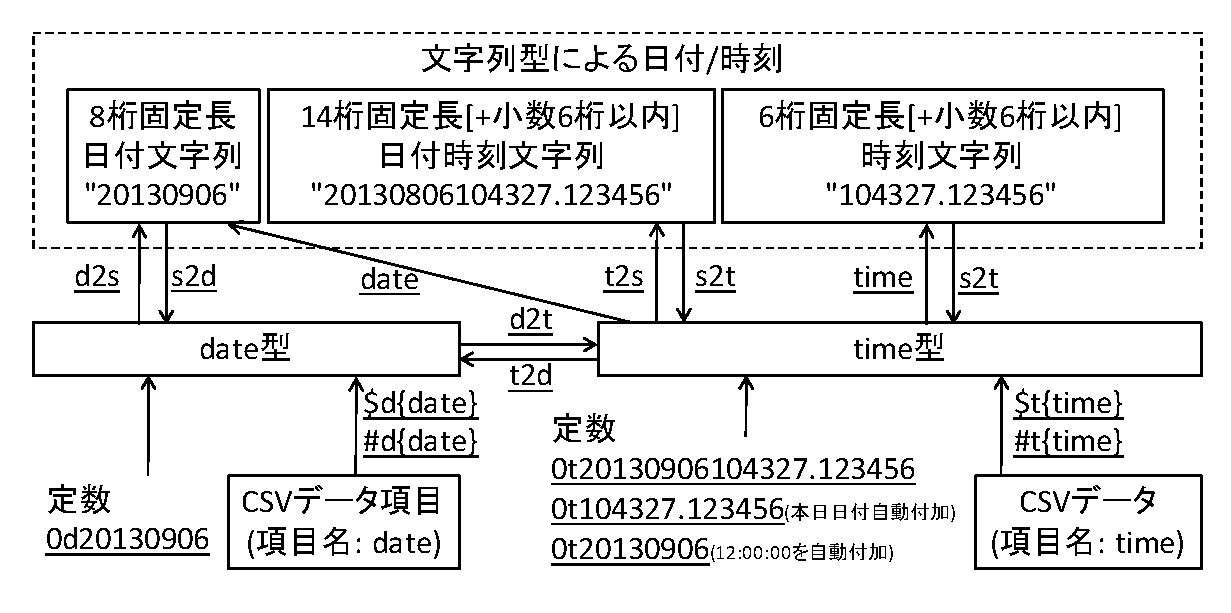
\includegraphics[scale=.50]{figure/datetime/datetime.eps}
\caption{2013年9月6日10時43分27秒を例に、date型とtime型と各種関数の関係を図示している。
実線で囲われたボックスは実データを表し、アンダーラインを付したものは関数等を表している。\label{fig:mcal_datetime}}
\end{center}
\end{figure}

またユーザは日付/時刻として固定長文字列を標準とせずに、
ユリウス通日(紀元前4713年1月1日正午からの日数)やUNIX時刻(1970年1月1日00時00分00秒(GMT)からの
経過秒数)などの整数を標準の日時の表記として利用してもよいであろう。
ユリウス通日やUNIX時刻と、日付型/時刻型との変換関数も備えており、十分に運用可能である。
ただし、mcalが提供する日付/時刻関数を使う限りにおいては、内部的にはグレゴリオ暦によって管理されており、
その範囲は、1400年1月1日から9999年12月31日に限定されることに注意する。
またUNIX時刻は32ビット整数で管理されているため、2038年1月19日3時14分7秒を超えると正しく計算できないことに注意する。
ただユリウス通日やUNIX時刻を利用する欠点は、その数字を見ただけでは実際にいつの日付時刻なのか理解出来ない点にあろう。

%\end{document}
